%!TEX root = main.tex


\section{Back-up}


\begin{frame}
\frametitle{A Large Ion Collider Experiement }
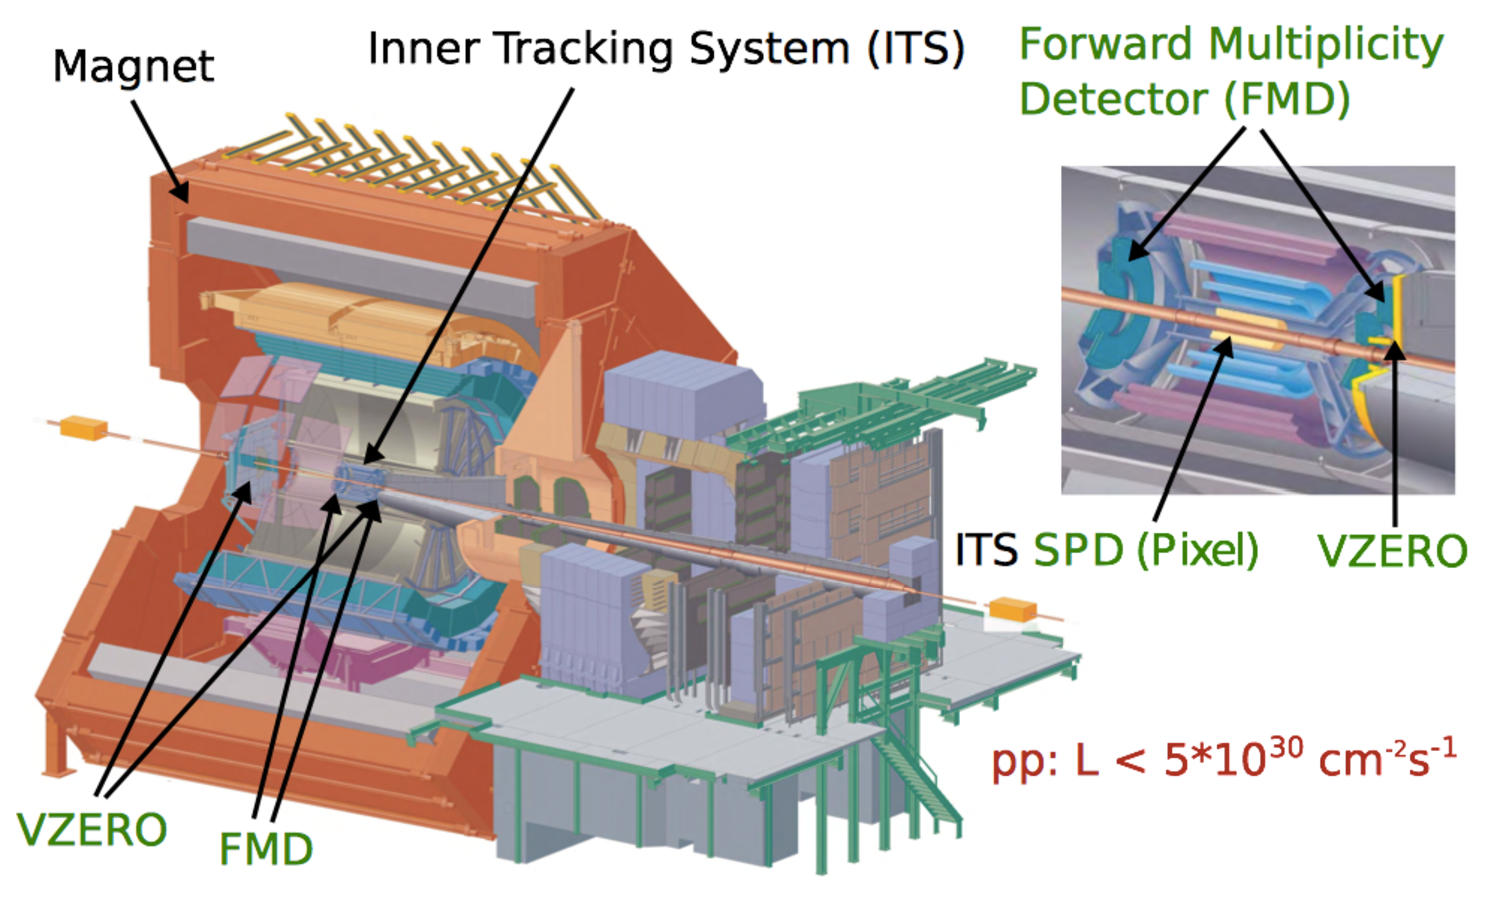
\includegraphics[width=1\linewidth]{ALICE}\\
\end{frame}

\begin{frame}
\frametitle{Diffraction}
Definition\\
: when the squared momentum transfer is much less than $\sqrt{s}$
\begin{columns}[c]
\column{.5\textwidth}
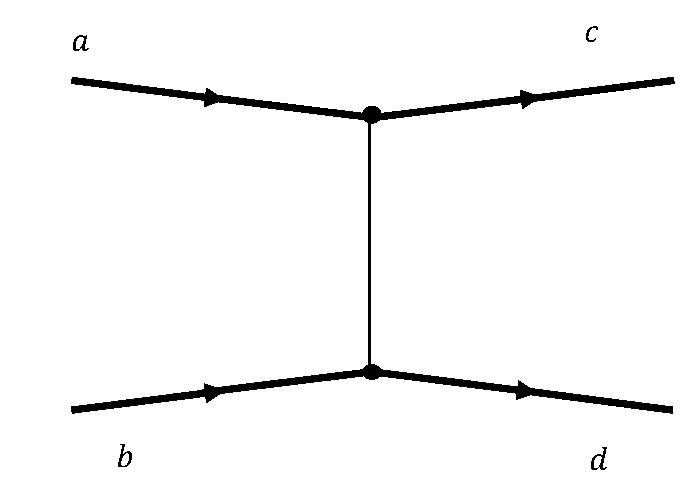
\includegraphics[width=1.\linewidth]{diffschematic}\\
\column{.5\textwidth}
$t = (p_\mathrm{a} - p_\mathrm{c})^2$ $\ll$ $\sqrt{s}$
\end{columns}
\begin{itemize}
\item{Help us understand QCD in the non-perturbative regime \\ (t $\sim$ 0 or $q^2$ $<$ $\mathrm{\Lambda}^2_\mathrm{QCD}$)}
\item{By Regge theory \footnotemark[1] \footnotemark[2] \footnotemark[3], diffraction proceeds via the exchange of Pomerons (${gg}_{\textrm{leading order}} + {ggg}_{\textrm{next leading order}} + \cdots$)}
\end{itemize}
\footnotetext[1]{P.D.B.Collins,An Introduction to Regge Theory and High Energy Physics, Cambridge, 1977}
\footnotetext[2]{A.B.Kaidalov,Phys.Rep.50,157,1979}
\footnotetext[3]{V. Barone, E. Predazzi, High-Energy Particle Diffraction ,Springer, Berlin, 200}
\end{frame}

\begin{frame}
\frametitle{Single Diffraction (SD)}
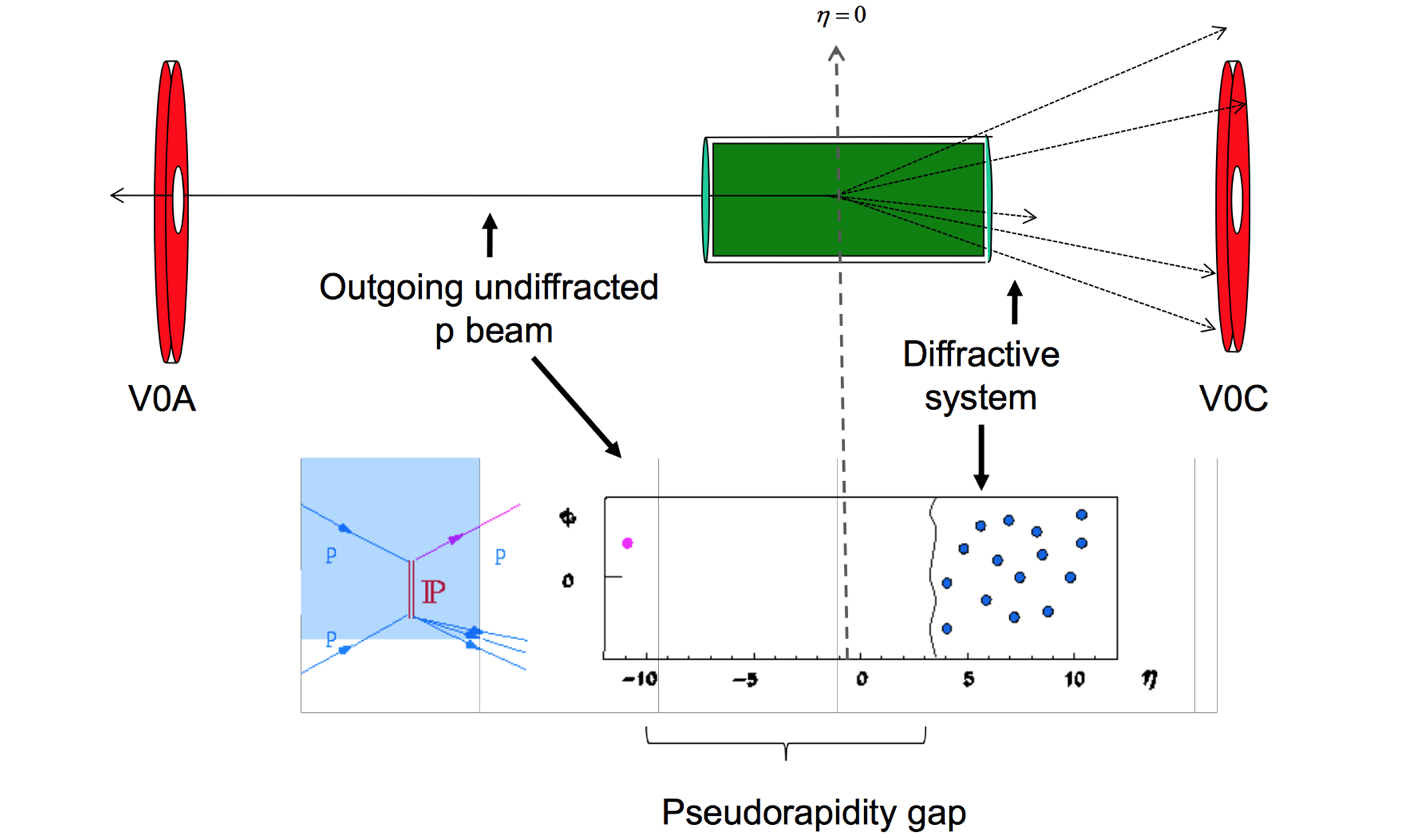
\includegraphics[width=1\linewidth]{sdschematic.png}\\
\end{frame}
\begin{frame}
\frametitle{Double Diffraction (DD)}
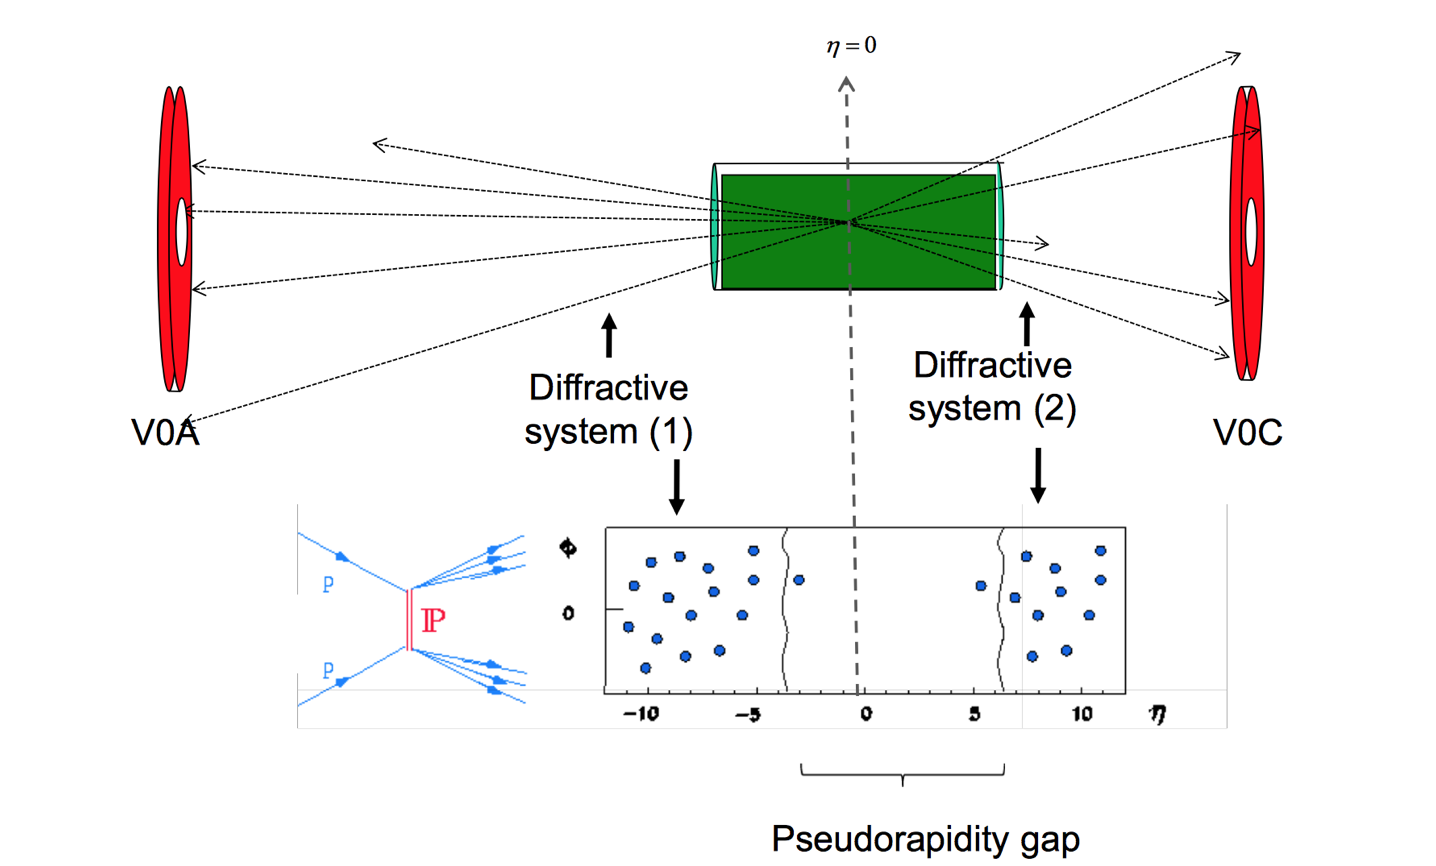
\includegraphics[width=1\linewidth]{ddschematic.png}\\
\end{frame}
\begin{frame}
\frametitle{Non Diffraction (ND)}
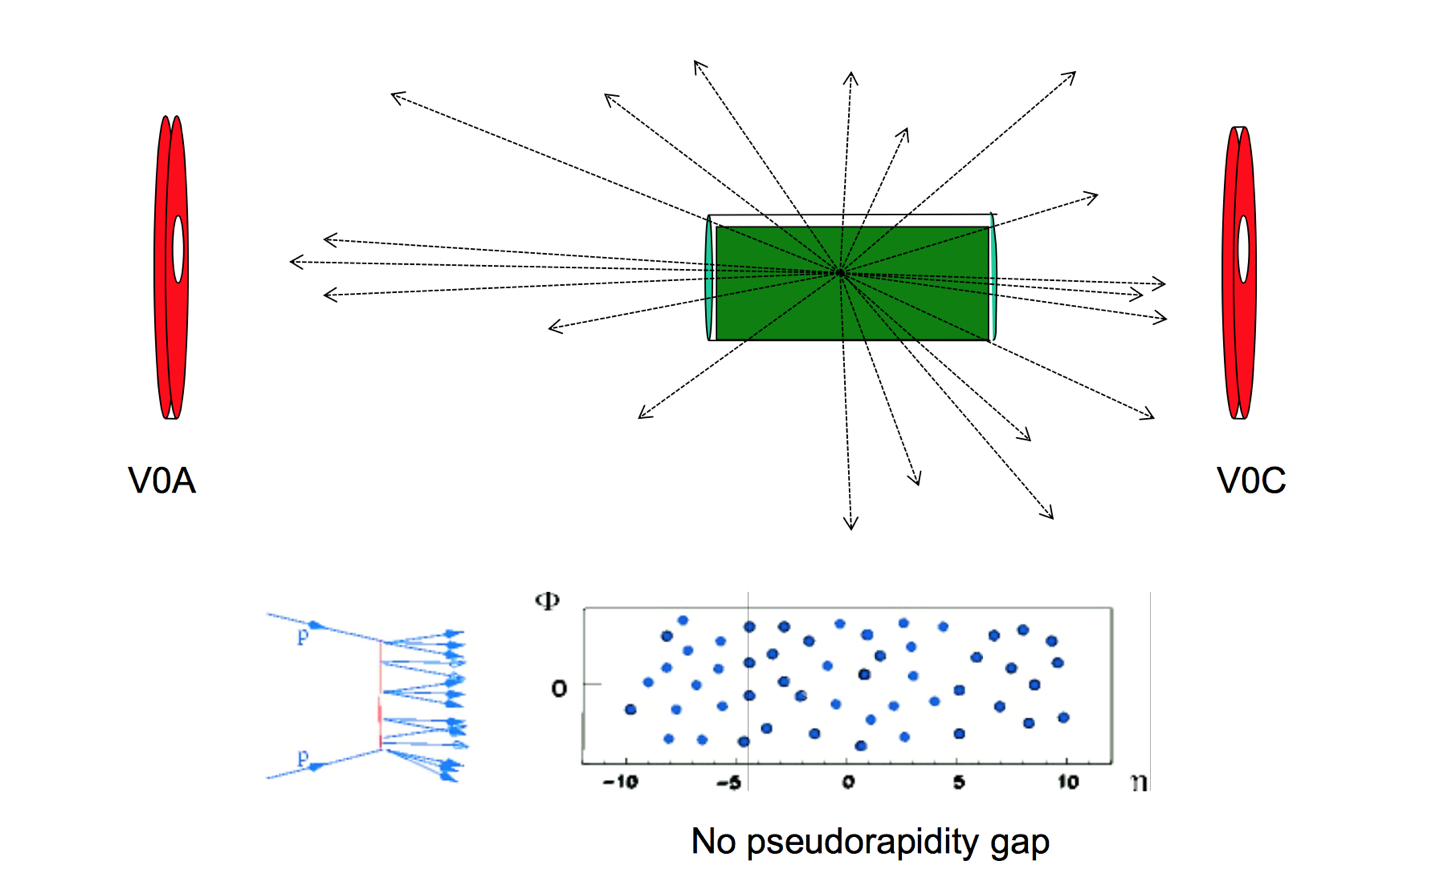
\includegraphics[width=1\linewidth]{ndschematic.png}\\
\end{frame}
\begin{frame}
\frametitle{Central Diffraction (CD)}
Central-diffractive event (theoretically ) \\= Double-rapidity-gap event (Experimentally)
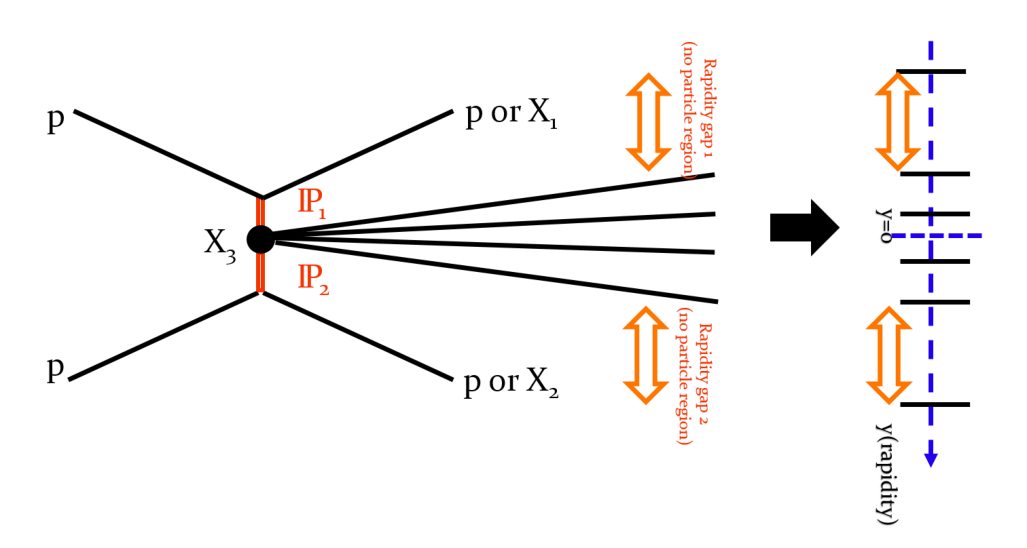
\includegraphics[width=1\linewidth]{cdschematic}\\
\end{frame}













